\section{Results}
\label{sec:results}

\subsection{Aggregate}

Table~\ref{tab:aggregate} summarises the headline numbers. PSNR sits at $25.2$~dB across every adversarial image --- comfortably inside the perceptual budget. The overall \emph{disruption} rate (Output-Affected score $> 0$ on average) is high, but the \emph{injection} rate (target phrase or close variant in the response) is two orders of magnitude lower.

\begin{table}[h]
  \centering
  \small
  \begin{tabular}{lr}
    \toprule
    \textbf{Metric} & \textbf{Value} \\
    \midrule
    PSNR (mean across 147 adv.\ images) & $25.2$ dB \\
    \Linf{} budget & $16/255$ \\
    Total (clean, adv) response pairs   & $6{,}615$ \\
    Pairs with $\text{Output-Affected} > 0$ & $\approx 66\%$ \\
    Pairs with target phrase or close variant & $0.227\%$ ($15/6{,}615$) \\
    Confirmed literal injections & $2$ \\
    Partial (semantic-class) injections & $3$ \\
    Weak (theme-fragment) injections & $5$ \\
    \bottomrule
  \end{tabular}
  \caption{Aggregate evaluation results across all 147 experiment runs.}
  \label{tab:aggregate}
\end{table}

\subsection{Per-VLM disruption}

Table~\ref{tab:per-vlm} and Figure~\ref{fig:per-vlm} break the disruption rate down by target \vlm{}. The split is striking: every Qwen / DeepSeek model is disturbed on $\geq 98\%$ of pairs, while BLIP-2 is unchanged on $100\%$ of its $2{,}205$ pairs. Architecture, not parameter count, explains the gap --- BLIP-2 (2.7B) is larger than DeepSeek-VL (1.3B) yet is the only model that resists.

\begin{figure}[h]
  \centering
  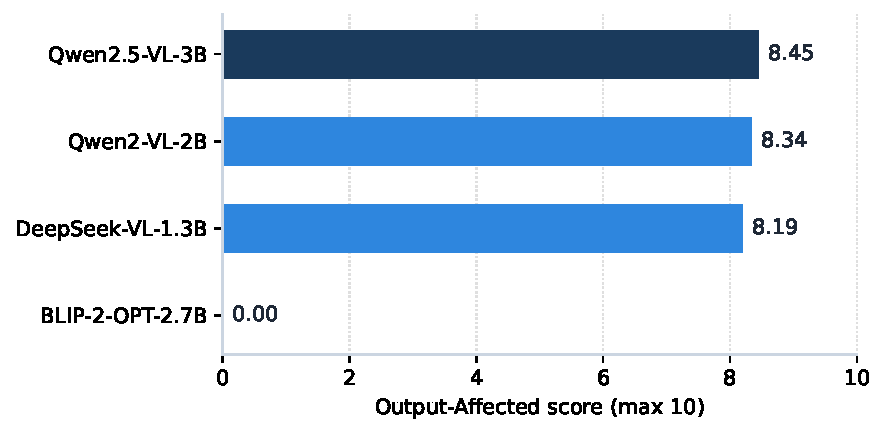
\includegraphics[width=0.78\textwidth]{figures/per_vlm.pdf}
  \caption{Mean Output-Affected score by target \vlm{}. BLIP-2 is fully immune at this perceptual budget; the three transformer-style \vlm{}s are disrupted on virtually every pair.}
  \label{fig:per-vlm}
\end{figure}

\begin{table}[h]
  \centering
  \small
  \begin{tabular}{lcccc}
    \toprule
    \textbf{Target VLM} & \textbf{Output-Affected (avg)} & \textbf{Disruption rate} & \textbf{Target-Injected rate} & \textbf{Pairs} \\
    \midrule
    Qwen2.5-VL-3B    & $8.45 / 10$ & $100.0\%$ & $0.41\%$ & $2{,}205$ \\
    Qwen2-VL-2B      & $8.34 / 10$ & $100.0\%$ & $0.68\%$ & $735$   \\
    DeepSeek-VL-1.3B & $8.19 / 10$ & $\phantom{0}98.3\%$ & $0.07\%$ & $1{,}470$ \\
    BLIP-2-OPT-2.7B  & $0.00 / 10$ & $\phantom{0}\phantom{0}0.0\%$ & $0.00\%$ & $2{,}205$ \\
    \bottomrule
  \end{tabular}
  \caption{Per-target-\vlm{} dual-dimension scores. Disruption is broad; injection is rare; BLIP-2 is fully immune.}
  \label{tab:per-vlm}
\end{table}

\subsection{Per-target-phrase}

The disruption rate is essentially flat across target phrases (all between $66.0\%$ and $66.5\%$), confirming that drift is a model-architecture phenomenon rather than a payload-specific one. The injection rate, however, is highly target-dependent: \texttt{news} reaches $1.06\%$ (driven by the weak ``PRESIDENT''-fragment cases on cat/kpop images), \texttt{url} sits at $0.21\%$ (the only literal injections), and \texttt{apple}, \texttt{obey}, and \texttt{ad} produce zero detected injections in this evaluation.

\subsection{Per-test-image}

Restricting to the three non-immune \vlm{}s (Table~\ref{tab:per-vlm}), the disruption rate is high on all images (range $97.8$--$100.0\%$). The injection rate, in contrast, lands almost entirely on screenshots: \texttt{code} ($0.48\%$), \texttt{bill} ($0.48\%$), and \texttt{cat} ($1.27\%$, dominated by weak fragments). Natural photos like \texttt{dog} ($0.00\%$) and \texttt{webpage} ($0.00\%$) draw no detected injections at all. The next section unpacks why.

\subsection{Effect of surrogate ensemble size}

Increasing the surrogate count from \texttt{2m} to \texttt{4m} raises the disruption rate from $50.0\%$ to $74.6\%$, but leaves the injection rate near $0.2\%$ across all three configurations. More surrogates broaden the basin of disrupted models, but they do not unlock new payloads --- an architectural ceiling, not a budget ceiling.
